\documentclass[../main.tex]{subfiles}
\begin{document}
\chapter{The Double-$\tau_h$ + jet trigger}

In view of Run 3, a lot of effort has been dedicated in order to maximize the collection efficiency from rare physics processes. In our case, we will try to increase the acceptance to the $H\to\tau\tau$ and $HH\to bb\tau\tau$ processes.

In most of the $H\to\tau\tau$ events used in the analysis, the $\tau\tau$ pair is accompanied by one or more jets coming from the hard-scattering processes or from QCD radiation (in addition to the 2 $b$-jets coming from the other $H$ in the $HH\to bb\tau\tau$ analysis), as seen in Fig.~\ref{hh:fig:trig_ngenjets}. In fact, most of the sensitivity in the $H\to\tau\tau$ analysis \cite{hh:htt_2016} comes from the categories with at least 1 jet. Therefore, by requiring at trigger level an additional jet on top of the already present double-$\tau_h$ trigger, the $p_t$ threshold on the $\tau_h$ could be lowered. By doing so, as more $\tau_h$ will be available for triggering (see Fig.~\ref{hh:fig:trig_l1tau_pt}), the acceptance of both analysis could be enlarged.


\begin{figure}[h!]
\begin{center}
\includegraphics[width=0.5\textwidth]{Images/ngenjet}
\end{center}
\caption{Number of jets  per event at generator level in a $H\to\tau\tau$ ggH simulated sample.}
\label{hh:fig:trig_ngenjets}
\end{figure}

\begin{figure}[h!]
\begin{center}
\includegraphics[width=0.5\textwidth]{Images/l1tau_pt}
\end{center}
\caption{L1 $\tau_h$ $p_t$ in a $H\to\tau\tau$ ggH simulated sample.}
\label{hh:fig:trig_l1tau_pt}
\end{figure}



\section{The L1 Double-$\tau_h$ + jet trigger}

\textcolor{red}{Shall we explain here what is the L1 menu or in the introduction? $\to$ Intro, leaving this here to remember}

At L1, the strategy we will follow is to include a new seed in the L1 Menu with two isolated $\tau_h$ objects and one jet object identified by the $\mu$GT in order to complement the already present \texttt{L1\_DoubleIsoTau32er2p1} seed, where two isolated $\tau_h$ with $p_t\geq32$~GeV and $|\eta|<2.1$ are considered, or even increase the $p_t$ threshold on this seed to keep the rate added as low as possible. However, a particular treatment has to be given to seeds involving $\tau_h$ and jet objects simultaneously, as both are reconstructed as purely calorimetric objects. Then, all $\tau_h$ objects will enter the L1 jet collection, while some of the L1 jets will also appear in the L1 $\tau_h$ collection. This issue can be perfectly seen in Fig.~\ref{hh:fig:l1_tau_jet_dR}. To reduce this effect, a feature called overlap removal \cite{intro:l1_13tev} is used, so only L1 jets that are separated more than $\Delta R>0.5$ with the selected $\tau_h$ are considered. This feature was present in the $\mu$GT before the inclusion of the seeds, although none of the already present seeds were using it and, in fact, it had to be tuned before attempting the inclusion of the new seeds.

\begin{figure}[h!]
\begin{center}
\includegraphics[width=0.5\textwidth]{Images/l1_tau_jet_dR}
\end{center}
\caption{Minimal $\Delta R$ between all L1 $\tau_h$'s and jets per event in a $H\to\tau\tau$ ggH simulated sample. The peak appearing at small $\Delta R$ values is due to the overlap between the L1 $\tau_h$ and jet collections.}
\label{hh:fig:l1_tau_jet_dR}
\end{figure}

This new double-$\tau_h$+jet seed (encoded as \texttt{L1\_Double\-IsoTauY\-er2p1\-\_JetZ\_RmOvlp\_dR0p5}) does not aim to replace the present \texttt{L1\_Double\-Iso\-Tau32er2p1} seed, but to complement it. However, increasing this double-$\tau_h$ threshold to a value $X$ could be needed in order to make some rate available to the new seed, so the double-$\tau_h$ seed gets encoded as \texttt{L1\_Double\-Iso\-TauXer2p1}. The rates corresponding to different values of the threshold $X$ are shown in Fig.~\ref{hh:fig:trig_ditau32_rate}, estimated using a zero bias data sample taken during a 2018 run but with Run-3 conditions applied (PU linearly scaled to 53 and 2748 colliding bunches). Among the possible sets of thresholds, we will consider only the ones that give a rate\,$\sim$\,15~kHz, compatible with the one given by \texttt{L1\_Double\-Iso\-Tau32er2p1}.


\begin{figure}[h!]
\begin{center}
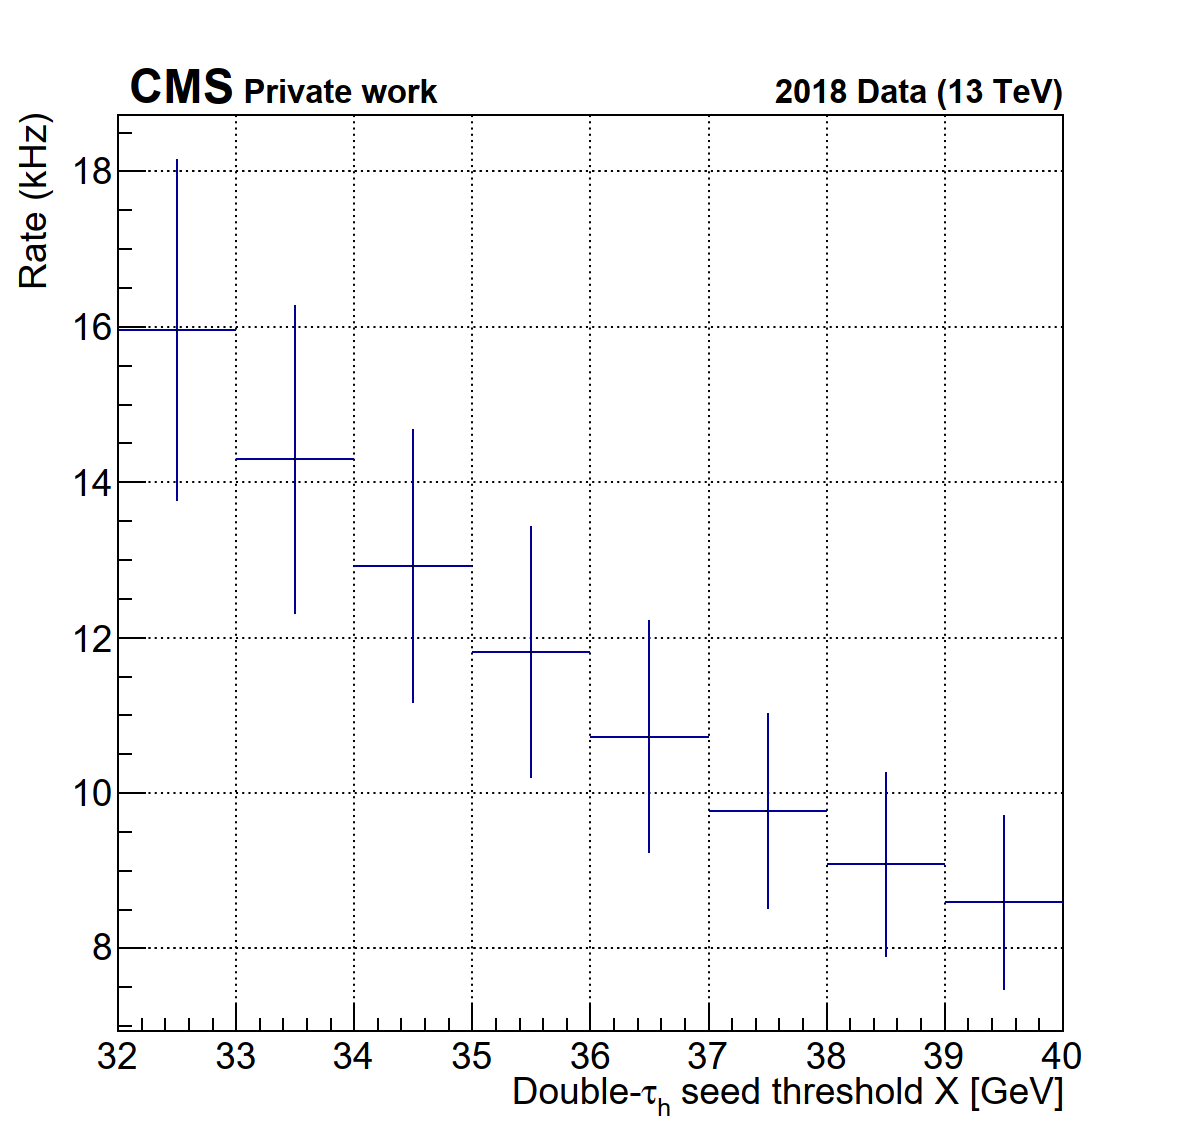
\includegraphics[width=0.5\textwidth]{Images/plot2D_ditau_sym_323755}
\end{center}
\caption{Rate of the \texttt{L1\_DoubleIsoTauXer2p1} trigger seed as a function of the $X$ threshold.}
\label{hh:fig:trig_ditau32_rate}
\end{figure}

As we would like to increase the signal acceptance, we will compute the acceptance gain when considering the two new seeds instead of the reference \texttt{L1\_DoubleIsoTau32er2p1} seed. In this case we will consider four signal samples, two ggH and VBFH $H\to\tau\tau$ and two ggHH and VBFHH $HH\to bb\tau\tau$. These acceptance gains are computed not only considering if the L1 objects pass the required selection cuts (grouped in the booleans \texttt{PassL1DoubleTau32}, \texttt{PassL1DoubleTauX} and \texttt{PassL1DoubleTauYJetZ}), but also applying selections to the objects obtained by the offline reconstruction system that evolve accordingly to the L1 thresholds considered. In general, this evolution means that, for a given L1 $p_t$ threshold $T$, the offline threshold is obtained as $T$ + $\Delta T$, where $\Delta T>0$ is a quantity that will depend on the analysis considered. For instance, in the $H\to\tau\tau$ analysis \cite{hh:htt_2016}, the leading $\tau_h$ is required to have a $p_t\geq 50$~GeV, while for the subleading this value drops to 40~GeV. Therefore, we will consider $\Delta X=\Delta Y=18$ GeV and $\Delta X=\Delta Y=8$ GeV for the leading and subleading $\tau_h$ respectively when obtaining the $H\to\tau\tau$ acceptance gains. In the $HH\to bb\tau\tau$ analysis \textcolor{red}{[paper when it's ready]} both $\tau_h$ are required to have a $p_t\geq40$~GeV, so we will set $\Delta X=\Delta Y=8$~GeV for both $\tau_h$. For the jets, we will consider $\Delta Z=10$~GeV for both analysis. Apart from this $p_t$ requirements, two different categorizations will be applied to the $H\to\tau\tau$ samples and one to the $HH\to bb\tau\tau$. Among the first ones we find the 1-jet, high $p_t$ category, where we consider events with one jet with $p_t\geq70$~GeV; and the 2-jet category, where we ask for two jets with $p_t\geq30$~GeV. In the $bb\tau\tau$ category we will just ask for 2 jets with $p_t\geq20$~GeV. All $p_t$ selections are summarised in Table~\ref{hh:tab:trig_offpt}, where one boolean associated to each of the seeds considered has been defined to group the needed selections. On top of these $p_t$ cuts, we ask all offline jets to have $|\eta|<4.7$ and pass tight jet ID and loose PU jet ID and an overlap removal criteria with the offline $\tau_h$.




\begin{table}
	\begin{center}
	\begin{tabular}{c || c | c | c }
		                           & \multicolumn{3}{c}{Offline $p_t$ selections} \\
		Boolean                    & 1-jet, high $p_t$ & 2-jet & bb$\tau\tau$ \\\hline\hline
		\texttt{PassOfflDoubleTau32} & 
			$\begin{matrix}
				p_t^{\tau_1}>50\\
				p_t^{\tau_2}>40\\
				p_t^{j_1}>70
			\end{matrix}$ &
			$\begin{matrix}
				p_t^{\tau_1}>50\\
				p_t^{\tau_2}>40\\
				p_t^{j_1}>30 \\
				p_t^{j_2}>30
			\end{matrix}$ &
			$\begin{matrix}
				p_t^{\tau_1}>40\\
				p_t^{\tau_2}>40\\
				p_t^{j_1}>20\\
				p_t^{j_2}>20
			\end{matrix}$ \\\hline
		\texttt{PassOfflDoubleTauX} & 
			$\begin{matrix}
				p_t^{\tau_1}>X+18\\
				p_t^{\tau_2}>X+8\\
				p_t^{j_1}>70
			\end{matrix}$ &
			$\begin{matrix}
				p_t^{\tau_1}>X+18\\
				p_t^{\tau_2}>X+8\\
				p_t^{j_1}>30 \\
				p_t^{j_2}>30
			\end{matrix}$ &
			$\begin{matrix}
				p_t^{\tau_1}>X+18\\
				p_t^{\tau_2}>X+8\\
				p_t^{j_1}>20\\
				p_t^{j_2}>20
			\end{matrix}$ \\\hline
		\texttt{PassOfflDoubleTauYJetZ} &
			$\begin{matrix}
				p_t^{\tau_1}>Y+18\\
				p_t^{\tau_2}>Y+8\\
				p_t^{j_1}>Z+10 \\
				p_t^{j_1}>70
			\end{matrix}$ &
			$\begin{matrix}
				p_t^{\tau_1}>Y+18\\
				p_t^{\tau_2}>Y+8\\
				p_t^{j_1}>Z+10 \\
				p_t^{j_1}>30 \\
				p_t^{j_2}>30
			\end{matrix}$ &
			$\begin{matrix}
				p_t^{\tau_1}>Y+8\\
				p_t^{\tau_2}>Y+8\\
				p_t^{j_1}>Z+10 \\
				p_t^{j_1}>20 \\
				p_t^{j_2}>20
			\end{matrix}$
	\end{tabular}
	\end{center}

	\caption{Offline $p_t$ selections associated to the L1 selections of \texttt{L1\_DoubleIsoTau32er2p1}, \texttt{L1\_DoubleIsoTauXer2p1} and \texttt{L1\_DoubleIsoTauYer2p1\_JetZ\_RmOvlp\_dR0p5}. All thresholds are expressed in GeV.}
	\label{hh:tab:trig_offpt}
\end{table}


Thus, the acceptance gain when adding a double-$\tau_h$+jet seed and modifying the threshold of the present double-$\tau_h$ seed can be defined as
\begin{equation}
g(X, Y, Z) = \frac{\begin{matrix}N[(\text{\texttt{PassL1DoubleTauX}} \,\,\&\&\,\, \text{\texttt{PassOfflDoubleTauX}}) \,\,||\,\, \\ \qquad\qquad\qquad(\text{\texttt{PassL1DoubleTauYJetZ}} \,\,\&\&\,\, \text{\texttt{PassOfflDoubleTauYJetZ}})] \end{matrix}}{N[\text{\texttt{PassL1DoubleTau32}} \,\,\&\&\,\, \text{\texttt{PassOfflDoubleTau32}}]}
\end{equation}
where $N$ is the number of events that pass the conditions required. The average acceptance gains for the samples and categories considered is shown in Fig.~\ref{hh:fig:l1_trig_mean_acc} (only the 20 sets with the highest acceptance gain in a 15-16 kHz rate range are displayed). Given these results, the decision was to consider thresholds $Y=26$ and $Z=55$ GeV for the double-$\tau_h$+jet seed. However, another double-$\tau_h$+jet seed with thresholds $Y=26$ GeV and $Z=70$ GeV was added a backup seed to account for possible high rate scenarios. Rates for these new seeds and their main acceptance gains on top of the \texttt{L1\_DoubleIsoTau32er2p1} seed are shown in Table~\ref{hh:tab:l1trig:allseeds}.

\begin{figure}
\centering\includegraphics[width=0.6\textwidth]{Images/rate_vs_mean_acceptance__min15.0___max16.0___xx_sym__yy_sym.pdf}

\caption{Mean acceptance gain for the samples and categories considered.}
\label{hh:fig:l1_trig_mean_acc}
\end{figure}

\begin{table}[h!]
\begin{center}
\begin{tabular}{|l|r|r|}
\hline
Trigger seed & Mean acceptance gain & Rate (kHz) \\\hline
\texttt{L1\_DoubleIsoTau26er2p1\_Jet55\_RmOvlp\_dR0p5} & 41$\%$& $8.3 \pm 2.8$ \\
\texttt{L1\_DoubleIsoTau26er2p1\_Jet70\_RmOvlp\_dR0p5} & 33$\%$& $5.3 \pm 1.8$ \\\hline
\end{tabular}
\end{center}

\caption{Rates and mean acceptance gains for the two new Double-$\tau_h$+jet seeds.}
\label{hh:tab:l1trig:allseeds}
\end{table}

%\begin{tabular}{|l|r|rr|rr|rr|r|}
%\hline
%\multicolumn{2}{|r|}{} & \multicolumn{2}{r|}{$H\to\tau\tau$, 1-jet, high $p_t$ cat.} & \multicolumn{2}{r|}{$H\to\tau\tau$, 2-jet cat.} & \multicolumn{2}{r|}{ $HH\to bb\tau\tau$} & \\\hline
% Parameters   &   Rate &    ggH &   VBFH &   ggH &  VBFH &   ggHH &   VBFHH &   Mean \\
%\hline
% 32,26,55     &  18.03 &                           1.50 &                           1.49 &                    1.35 &                    1.43 &           1.29 &           1.42 &   1.41 \\
% 32,26,70     &  16.42 &                           1.37 &                           1.38 &                    1.27 &                    1.34 &           1.25 &           1.34 &   1.33 \\
% 35,26,55     &  15.34 &                           1.47 &                           1.47 &                    1.29 &                    1.39 &           1.27 &           1.39 &   1.38 \\
% 35,26,70     &  13.27 &                           1.31 &                           1.33 &                    1.18 &                    1.27 &           1.20 &           1.28 &   1.26 \\
%\hline
%\end{tabular}


\section{The L1 Double-$\tau_h$ + jet trigger online performance}

\textcolor{red}{Fill with rates comparing online/L1 Menu Tools, acceptance gains w.r.t DoubleIsoTau32 alone}


\section{The HLT Double-$\tau_h$ + jet paths}




\bibliographystyle{plain}
\bibliography{../biblio.bib}





\end{document}

